\documentclass[a4paper]{report}

%================================
% PACKAGE IMPORTS
%================================

% Basic packages
\usepackage{graphicx} % For including images
\usepackage[utf8]{inputenc} % Document encoding
\usepackage[T1]{fontenc} % Font encoding
\usepackage{titling} % Customizing the title
\usepackage[italian]{babel} % Main language of the document

\usepackage{longtable} 
\usepackage{tabularx}
\usepackage{booktabs}

% Mathematical packages
\usepackage{amsmath, amssymb, amsthm, mathtools} % Standard math packages

% Hyperlink packages
\usepackage{hyperref} % Handling hyperlinks in the document

% Layout and formatting packages
\usepackage{geometry} % Page dimensions and margin setup
\usepackage{fancyhdr} % Customizing headers and footers
\usepackage{xcolor} % Color management in the document
\usepackage[table]{xcolor}
\usepackage{wrapfig} % Wrapping figures in text
\usepackage{array} % Enhancements for tables
\usepackage{float} % Force table placement with [H]
\usepackage{varwidth} % Variable-width columns

% Advanced packages
\usepackage{tikz} % Drawing graphs and diagrams
\usepackage{amsmath, siunitx}
\usepackage{circuitikz}
\usetikzlibrary{arrows.meta, decorations.pathreplacing, positioning, calc, backgrounds}
\usepackage{pgfplots} % Plotting data and functions
\usepackage{titlesec} % Customizing section titles
\usepackage{titletoc} % Customizing table of contents
\usepackage{fix-cm} % Fixing font size issues

% Advanced math packages
\usepackage[varbb]{newpxmath} % Advanced math font style
\usepackage{xfrac} % Inclined fractions
\usepackage[makeroom]{cancel} % Canceling terms in equations
\usepackage{stmaryrd} % To use the \lightning symbol

% Document management packages
\usepackage{bookmark} % Handling bookmarks in PDF files
\usepackage{enumitem} % Customizing lists
\usepackage{theoremref} % Cross-references for theorems and propositions

% Additional packages
\usepackage[most, many, breakable]{tcolorbox} % Customizable colored boxes
\usepackage{etoolbox} % Tools for command modifications
\usepackage{caption} % control caption alignment for tables
\usepackage{enumitem} % control list layout and labels
\usepackage{nameref} % Cross-references for names
\usepackage{multicol} % Multi-column layout
\usepackage{tikz} % To circle items
\usepackage{tikz-cd} % Commutative diagrams
\usepackage[ruled, vlined, linesnumbered]{algorithm2e} % Algorithms and pseudocode
\usepackage{comment} % Multi-line comments
\usepackage{import} % Importing documents from other folders
\usepackage{xifthen} % Conditional commands
\usepackage{pdfpages} % Including external PDF pages
\usepackage{transparent} % Transparency in graphic elements

% PDF
\usepackage{pdfpages}

% Starred commands
\usepackage{suffix}

%================================
% TABLE SETTINGS
%================================
\setlength{\arrayrulewidth}{0.5mm}
\setlength{\tabcolsep}{14pt}
\renewcommand{\arraystretch}{2.5}

% Make longtable flush-left by default when its natural width is smaller than \textwidth
% longtable centers tables using \LTleft and \LTright; set them to 0 to align left
\setlength{\LTleft}{0pt}
\setlength{\LTright}{0pt}

% Make standard table floats left-aligned (even if they contain \centering)
% - captions: disable singleline centering and use raggedright justification
% - AtBeginEnvironment: apply raggedright and locally neutralize \centering
\captionsetup[table]{singlelinecheck=false, justification=raggedright}
\AtBeginEnvironment{table}{\raggedright\let\centering\relax}

%================================
% TABLE OF CONTENTS SETTINGS
%================================
\renewcommand\thesection{\arabic{section}}
\titlecontents{chapter}[1.05em]{\bigskip}%
{\contentslabel[\MakeUppercase{\romannumeral\thecontentslabel}]{1em}\enspace\textsc}%
{\hspace*{-1em}\textsc}%
{\hfill\contentspage}%
\titlecontents{section}[1.6em]{\smallskip}%
{\thecontentslabel.\enspace}{}%
{\titlerule*[1pc]{.}\contentspage}%
\setcounter{tocdepth}{3}

% Import the images contained in the img folder
\graphicspath{{./img/}}

%================================
% HEADER AND FOOTER SETTINGS
%================================
\setlength{\headheight}{15pt}
\addtolength{\topmargin}{-2.5pt}
\setlength{\footskip}{15pt} % Set the footskip to a larger value
\pagestyle{fancy}
\fancyhf{}
\pretitle{\begin{center}\LARGE\bfseries}
		\posttitle{\end{center}}
\renewcommand{\headrulewidth}{0.5pt}
% Impostazione statica per l'intestazione a destra: mostra sempre il testo richiesto
% (in precedenza veniva impostato dinamicamente il titolo della sezione nei comandi custom)
\fancyhead[R]{\makebox[\textwidth][r]{Ingegneria del Software - Univpm}}
% Ensure header/footer span the same width as the main text and align to its right margin
% Sometimes fancyhdr's headwidth can be inconsistent; force it to the text width
\setlength{\headwidth}{\textwidth}
% Place the page number flush-right with respect to the text block
\fancyfoot[R]{\makebox[\textwidth][r]{\thepage}}

% Ensure the headrule (the horizontal line under the header) spans the text block
% and is left-aligned with the text margins.
\makeatletter
\renewcommand{\headrule}{%
	% draw a rule exactly \textwidth wide at the header thickness
	\hrule height \headrulewidth width \textwidth\vskip-\headrulewidth
}
\makeatother

%================================
% PAGE GEOMETRY SETTINGS
%================================
\geometry{margin=1in}

%================================
% HYPERLINK SETTINGS
%================================
\hypersetup{
	colorlinks=true,
	linkcolor=black,
	urlcolor=cyan,
	citecolor=black,
	filecolor=magenta,
	pdftitle={PDF Title},
}

%================================
% TCOLORBOX SETUPS
%================================

% THEOREM BOXES
\tcbuselibrary{theorems,skins,hooks}

\newtcolorbox[number within=section]{Theorem_blue}[2][]
{%
	enhanced,
	breakable,
	colback = thm_box_blue!5,
	frame hidden,
	boxrule = 0sp,
	borderline west = {2pt}{0pt}{thm_box_blue},
	sharp corners,
	detach title,
	before upper = \tcbtitle\par\smallskip,
	coltitle = thm_box_blue,
	fonttitle = \bfseries\sffamily,
	description font = \mdseries,
	separator sign none,
	segmentation style={solid, thm_box_blue},
	title = {#2},#1
}

\newtcolorbox[number within=section]{Theorem_yellow}[2][]
{%
	enhanced,
	breakable,
	colback = thm_box_yellow!5,
	frame hidden,
	boxrule = 0sp,
	borderline west = {2pt}{0pt}{thm_box_yellow},
	sharp corners,
	detach title,
	before upper = \tcbtitle\par\smallskip,
	coltitle = thm_box_yellow,
	fonttitle = \bfseries\sffamily,
	description font = \mdseries,
	separator sign none,
	segmentation style={solid, thm_box_yellow},
	title = {#2},#1
}

\newtcolorbox[number within=section]{Theorem_purple}[2][]
{%
	enhanced,
	breakable,
	colback = thm_box_purple!5,
	frame hidden,
	boxrule = 0sp,
	borderline west = {2pt}{0pt}{thm_box_purple},
	sharp corners,
	detach title,
	before upper = \tcbtitle\par\smallskip,
	coltitle = thm_box_purple,
	fonttitle = \bfseries\sffamily,
	description font = \mdseries,
	separator sign none,
	segmentation style={solid, thm_box_purple},
	title = {#2},#1
}

\newtcolorbox[number within=section]{Theorem_green}[2][]
{%
	enhanced,
	breakable,
	colback = thm_box_green!5,
	frame hidden,
	boxrule = 0sp,
	borderline west = {2pt}{0pt}{thm_box_green},
	sharp corners,
	detach title,
	before upper = \tcbtitle\par\smallskip,
	coltitle = thm_box_green,
	fonttitle = \bfseries\sffamily,
	description font = \mdseries,
	separator sign none,
	segmentation style={solid, thm_box_green},
	title = {#2},#1
}

% EXAMPLE BOX
\newtcolorbox[number within=section]{Example}[2][]
{%
	colback = example_box_clr!5,
	breakable,
	colframe = example_box_clr,
	coltitle = example_box_clr,
	boxrule = 1pt,
	sharp corners,
	detach title,
	before upper=\tcbtitle\par\smallskip,
	fonttitle = \bfseries,
	description font = \mdseries,
	separator sign none,
	description delimiters parenthesis,
	title = {#2},#1
}

% DEFINITION BOX
\newtcolorbox[number within=section]{Definition}[2][]{enhanced,
	before skip=2mm,after skip=2mm,
	colback=description_box_clr!5,
	colframe=description_box_clr,
	boxrule=0.5mm,
	attach boxed title to top left={xshift=1cm,yshift*=1mm-\tcboxedtitleheight},
	varwidth boxed title*=-3cm,
	boxed title style={frame code={
					\path[fill=description_box_clr]
					([yshift=-1mm,xshift=-1mm]frame.north west)
					arc[start angle=0,end angle=180,radius=1mm]
					([yshift=-1mm,xshift=1mm]frame.north east)
					arc[start angle=180,end angle=0,radius=1mm];
					\path[left color=description_box_clr!60!black,right color=description_box_clr!60!black,
						middle color=description_box_clr!80!black]
					([xshift=-2mm]frame.north west) -- ([xshift=2mm]frame.north east)
					[rounded corners=1mm]-- ([xshift=1mm,yshift=-1mm]frame.north east)
					-- (frame.south east) -- (frame.south west)
					-- ([xshift=-1mm,yshift=-1mm]frame.north west)
					[sharp corners]-- cycle;
				},interior engine=empty,
		},
	fonttitle=\bfseries,
	title={#2},#1}

% NOTE BOX
\usetikzlibrary{arrows,calc,shadows.blur}
\tcbuselibrary{skins}

\newtcolorbox{note}[1][]{%
	enhanced jigsaw,
	colback=gray!20!white,%
	colframe=gray!80!black,
	size=small,
	boxrule=1pt,
	title=\textbf{Nota:},
	halign title=flush center,
	coltitle=black,
	breakable,
	drop shadow=black!50!white,
	attach boxed title to top left={xshift=1cm,yshift=-\tcboxedtitleheight/2,yshifttext=-\tcboxedtitleheight/2},
	minipage boxed title=1.5cm,
	boxed title style={%
			colback=white,
			size=fbox,
			boxrule=1pt,
			boxsep=2pt,
			underlay={%
					\coordinate (dotA) at ($(interior.west) + (-0.5pt,0)$);
					\coordinate (dotB) at ($(interior.east) + (0.5pt,0)$);
					\begin{scope}
						\clip (interior.north west) rectangle ([xshift=3ex]interior.east);
						\filldraw [white, blur shadow={shadow opacity=60, shadow yshift=-.75ex}, rounded corners=2pt] (interior.north west) rectangle (interior.south east);
					\end{scope}
					\begin{scope}[gray!80!black]
						\fill (dotA) circle (2pt);
						\fill (dotB) circle (2pt);
					\end{scope}
				},
		},
	#1,
}

% MY BOX
\makeatletter
\newtcolorbox{mybox}[2][]{
	enhanced,
	breakable,
	colback=white,
	colframe=my_box_clr,
	attach boxed title to top left={yshift*=-\tcboxedtitleheight},
	fonttitle=\bfseries,
	title={#2},
	boxed title style={%
			sharp corners,
			rounded corners=northwest,
			colback=tcbcolframe,
			boxrule=0pt,
		},
	underlay boxed title={%
			\path[fill=tcbcolframe] (title.south west)--(title.south east)
			to[out=0, in=180] ([xshift=5mm]title.east)--
			(title.center-|frame.east)
			[rounded corners=\kvtcb@arc] |-
			(frame.north) -| cycle;
		},
	#1
}
\makeatother

%================================
% SELF MADE COMMANDS
%================================

\newcommand*\circled[1]{\tikz[baseline=(char.base)]{
		\node[shape=circle,draw,inner sep=1pt] (char) {#1};}}

% TColorBox commands
\newcommand{\thmbl}[2]{\begin{Theorem_blue}{#1}{}#2\end{Theorem_blue}}
\newcommand{\thmyllw}[2]{\begin{Theorem_yellow}{#1}{}#2\end{Theorem_yellow}}
\newcommand{\thmprpl}[2]{\begin{Theorem_purple}{#1}{}#2\end{Theorem_purple}}
\newcommand{\thmgrn}[2]{\begin{Theorem_green}{#1}{}#2\end{Theorem_green}}
\newcommand{\ex}[2]{\begin{Example}{#1}{}#2\end{Example}}
\newcommand{\dfn}[2]{\begin{Definition}[colbacktitle=red!75!black]{#1}{}#2\end{Definition}}
\newcommand{\nt}[1]{\begin{note}#1\end{note}}
\newcommand{\genericbox}[2]{\begin{mybox}{#1}{}#2\end{mybox}}

% Custom commands for chapters, sections, and subsections
\newcommand{\newchapter}[1]{%
	\newpage
	\phantomsection
	% Place chapter header flush-left with the text block
	\fancyhead[L]{\makebox[\textwidth][l]{#1}}%
	\chapter*{\textcolor{myColor}{#1}}
	\addcontentsline{toc}{chapter}{#1}%
	\thispagestyle{fancy}
}

%================================
% Adjust chapter spacing for both numbered and starred forms
%================================
% The document uses \chapter* via the custom \newchapter macro. Some
% spacing commands only affect the unstarred \chapter. To ensure both
% starred and unstarred chapters are moved closer to the top margin,
% prepend a small negative vertical space to the internal chapter macros.
% Tweak the -10pt value to taste.
\makeatletter
% Prepend negative vertical space before numbered and starred chapter heads
\pretocmd{\@chapter}{\vspace*{-60pt}}{}{}
\pretocmd{\@schapter}{\vspace*{-60pt}}{}{}
\makeatother

\newcommand{\newsection}[1]{%
	\phantomsection
	\section*{\textcolor{myColor}{#1}}%
	% Place section header flush-right with the text block
	% \fancyhead[R]{\makebox[\textwidth][r]{#1}}% <- originale commentato: non vogliamo più mostrare il titolo della sezione qui
	\addcontentsline{toc}{section}{#1}%
	\thispagestyle{fancy}
}

\newcommand{\newsubsection}[1]{%
	\phantomsection
	\subsection*{\textcolor{myColor}{#1}}%
	\addcontentsline{toc}{subsection}{#1}%
	\thispagestyle{fancy}
}

\newcommand{\newsubsubsection}[1]{%
	\phantomsection
	\subsubsection*{\textcolor{myColor}{#1}}%
	\addcontentsline{toc}{subsubsection}{#1}%
	\thispagestyle{fancy}
}

\WithSuffix\newcommand\newsection*[1]{%
	\phantomsection
	\section*{\textcolor{myColor}{#1}}%
	% Place section header flush-right with the text block
	% \fancyhead[R]{\makebox[\textwidth][r]{#1}}% <- originale commentato
	\thispagestyle{fancy}
}
\WithSuffix\newcommand\newsubsection*[1]{%
	\phantomsection
	\subsection*{\textcolor{myColor}{#1}}%
	\thispagestyle{fancy}
}

\WithSuffix\newcommand\newsubsubsection*[1]{%
	\phantomsection
	\subsubsection*{\textcolor{myColor}{#1}}%
	\thispagestyle{fancy}
}

%================================
% CUSTOM COLORS
%================================
\definecolor{highlighter}{RGB}{255,255,153}

\definecolor{description_box_clr}{RGB}{97,97,97}

\definecolor{thm_box_yellow}{RGB}{169,121,69}
\definecolor{thm_box_blue}{HTML}{00007B}
\definecolor{thm_box_purple}{RGB}{197, 92, 212}
\definecolor{thm_box_green}{RGB}{56, 140, 70}

\definecolor{example_box_clr}{HTML}{88D6D1}

\definecolor{my_box_clr}{HTML}{24598e}

\definecolor{myColor}{HTML}{242627}



%================================
% CUSTOM CODE SECTION
%================================
\usepackage{xcolor}

\definecolor{keywordviolet}{rgb}{0.6, 0.0, 0.8}   % viola acceso per keyword
\definecolor{commentgreen}{rgb}{0.0, 0.6, 0.2}    % verde brillante per commenti
\definecolor{stringorange}{rgb}{1.0, 0.5, 0.0}    % arancione acceso per stringhe
\definecolor{docstringblue}{rgb}{0.0, 0.4, 1.0}   % blu vivace per docstring
\definecolor{lightgraybg}{rgb}{0.95, 0.95, 0.95}  % grigio chiaro come sfondo
\renewcommand{\lstlistingname}{Unit Test}

\newcommand{\estiloPython}{
\lstset{
    language=Python,
    basicstyle=\ttfamily\small,
    keywordstyle=\color{keywordviolet}\bfseries,
    stringstyle=\color{stringorange},
    commentstyle=\color{commentgreen},
    morecomment=[s][\color{docstringblue}]{""" }{ """}, % docstring
    extendedchars=true,
    showspaces=false,
    showstringspaces=false,
    numbers=left,
    numberstyle=\tiny\color{gray},
    breaklines=true,
    backgroundcolor=\color{lightgraybg},
    breakautoindent=true,
    captionpos=b,
    xleftmargin=0pt,
    tabsize=2,
    escapeinside={\%*}{*)},
    morekeywords={self, setUp, Client, objects, create} % aggiungi altre keyword Django/Python
}}

% Document title and author
\title{\huge \textbf{\textcolor{black}{Elettromagnetismo\\per la Trasmissione dell'Informazione}}\\}
\author{Davide Ronchini - 2025}
\date{}

\begin{document}

\thispagestyle{empty} % rimuove intestazione/piede pagina

% decorative thin left band (1.2cm) drawn in overlay so it doesn't change layout
\begin{tikzpicture}[remember picture,overlay]
    % extend a couple millimetres below the page bottom to avoid any tiny gap
    \fill[myGreen] (current page.north west) rectangle ($(current page.south west)+(1.4cm,0)$);
\end{tikzpicture}

\begin{center}
    % Titolo Università
    \vphantom{space} \\[0.5cm]
    {\Large \textbf{\textcolor{myGreen}{GESTRI – Gestionale Rifiuti Industriali}}}\\[0.3cm]
    
    % Corso di Laurea
    {\normalsize Corso di Laurea Triennale in Ingegneria Informatica e dell’Automazione}\\[2cm]
    
    % Logo
    
\includegraphics[width=0.35\textwidth]{univpm_logo.png}\\[2cm]
    
    % Titolo progetto
    {\large \textbf{\textcolor{myGreen}{UNIVERSITÀ POLITECNICA DELLE MARCHE}}}\\ [0.3cm]
    % Corso di Laurea
    {\normalsize Corso di Laurea Triennale in Ingegneria Informatica e dell’Automazione}\\[2cm]
    
    % Relatori e Tesina
    \begin{minipage}{0.45\textwidth}
        \begin{flushleft}
        \textbf{\textcolor{myGreen}{RELATORI:}}\\[0.2cm]
        Prof. Ursino Domenico\\
        Prof. Davide Traini
        \end{flushleft}
    \end{minipage}
    \hfill
    \begin{minipage}{0.45\textwidth}
        \begin{flushright}
        \textbf{\textcolor{myGreen}{TESINA DI:}}\\[0.2cm]
        Tarek Naja \\
        Davide Ronchini\\
        Marco Sambughi \\
        Sara Vaccaro
        \end{flushright}
    \end{minipage}\\[5.5cm]
    
    % Anno accademico
    {\normalsize A.A 2024/2025}
\end{center}

% Include the table of contents
\tableofcontents
% Remove page number from table of contents page
\thispagestyle{empty}

\setcounter{page}{0}
\newchapter{Descrizione del Progetto}

\newsection{Panoramica Generale}
Il progetto si inserisce all’interno del contesto della gestione di un sistema avanzato destinato al monitoraggio e al controllo di un insieme complesso di dati e processi. 
L’obiettivo principale è fornire un’infrastruttura affidabile e centralizzata, capace di gestire in maniera integrata le informazioni provenienti da più fonti e di garantire 
un accesso sicuro e differenziato in base ai ruoli degli utenti.  
Il sistema non si limita alla sola raccolta dei dati, ma prevede una loro elaborazione, archiviazione e presentazione attraverso interfacce chiare e coerenti, 
con particolare attenzione alla scalabilità e alla manutenibilità futura.

\newsection{Utenti}
Gli utenti del sistema sono suddivisi in due categorie principali.  
La prima è quella degli \textbf{Operatori}, figure incaricate dell’inserimento e dell’aggiornamento delle informazioni di base, che costituiscono il nucleo operativo della piattaforma.  
La seconda è rappresentata dallo \textbf{Staff}, che eredita tutte le funzionalità proprie degli Operatori ma dispone inoltre di strumenti aggiuntivi per il monitoraggio, 
la supervisione e la gestione delle configurazioni globali del sistema.  
Per riassumere in modo uniforme le logiche comuni, è stato introdotto un attore generico denominato \textbf{User}, che rappresenta un’astrazione dei comportamenti condivisi 
tra tutte le tipologie di utenti.

\newsection{Gestione dei Dati}
Uno dei cardini del progetto è la gestione strutturata dei dati.  
Il sistema deve infatti raccogliere informazioni eterogenee, archiviarle in modo sicuro e consentirne il recupero secondo criteri di rapidità ed efficienza.  
Sono previsti meccanismi di aggiornamento costante e di sincronizzazione, così da garantire la coerenza delle informazioni nel tempo.  
Particolare attenzione è stata posta anche agli aspetti di integrità e consistenza, evitando ridondanze superflue e introducendo controlli atti a prevenire errori nella fase di registrazione.

\newsection{Architettura del Sistema}
L’architettura del sistema è stata progettata seguendo un approccio modulare, che consente di distinguere chiaramente i diversi livelli funzionali.  
Il livello di acquisizione si occupa di raccogliere i dati dalle fonti esterne, normalizzandoli e predisponendoli all’elaborazione.  
Segue un livello logico-gestionale, in cui le informazioni vengono trattate secondo le regole definite dal dominio applicativo.  
Infine, il livello di presentazione ha il compito di fornire agli utenti una visione chiara e comprensibile dello stato del sistema, adattandosi ai privilegi associati a ciascun ruolo.  
La modularità facilita inoltre l’eventuale estensione futura, consentendo di aggiungere nuove funzionalità senza compromettere la stabilità delle componenti esistenti.

\newsection{Interfacce e Accesso}
L’accesso al sistema avviene attraverso interfacce pensate per essere intuitive e coerenti, in grado di fornire a ciascun utente esattamente le funzioni necessarie al proprio ruolo.  
Gli Operatori interagiscono principalmente con strumenti di inserimento e aggiornamento, mentre lo Staff dispone di viste aggiuntive che consentono una supervisione complessiva.  
La gestione delle credenziali garantisce la distinzione tra i diversi profili, rafforzando il livello di sicurezza e impedendo utilizzi impropri delle funzionalità disponibili.


\newchapter{Glossario dei Termini}

\begin{longtable}{ >{\raggedright\arraybackslash}p{1.5cm} >{\raggedright\arraybackslash}p{5.5cm} >{\raggedright\arraybackslash}p{2cm} >{\raggedright\arraybackslash}p{2.97cm}}
\toprule
\textbf{TERMINE} & \textbf{DESCRIZIONE} & \textbf{TIPO} & \textbf{SINONIMI} \\
\midrule
\endhead
\bottomrule
\endfoot
\endlastfoot
Utente & Ruolo generico da cui derivano Client e Operator. Ha la capacità di accedere al sistema. & TECNICO & - \\
Client & Soggetto che commissiona il servizio e consulta documenti e stato delle attività. & BUSINESS & - \\
Operator & Figura incaricata di eseguire operazioni pratiche di carico/scarico, compilazione documenti e gestione mezzi. Estende le funzionalità dello Staff. & BUSINESS & - \\
Staff & Personale amministrativo che gestisce l'organizzazione dei turni, le assenze e le attività complessive. & BUSINESS & - \\
Attività & Operazione di carico o scarico di rifiuti, con assegnazione di operatori e mezzi. & BUSINESS & - \\
Mezzo & Veicolo utilizzato per il trasporto dei rifiuti. & BUSINESS & - \\
FIR & Documento obbligatorio che accompagna il trasporto dei rifiuti industriali. & BUSINESS & Formulario di Identificazione Rifiuti \\
Turno & Periodo temporale in cui un operatore è assegnato a un'attività. & BUSINESS & - \\
Gestione Utenti & Area del sistema che si occupa di registrazione, login, e amministrazione dei profili utente. & TECNICO & - \\
Gestione Attività & Area del sistema che gestisce la creazione, l'aggiornamento e il monitoraggio delle operazioni di carico/scarico rifiuti. & TECNICO & - \\
Gestione Documento & Area del sistema che gestisce la creazione, archiviazione e notifica di documenti come il FIR. & TECNICO & - \\
Gestione Mezzo & Area del sistema che tiene traccia dei dati tecnici, assicurativi e di manutenzione dei veicoli. & TECNICO & - \\
MoSCoW & Criterio di prioritizzazione dei requisiti: Must, Should, Could, Won't. & TECNICO & - \\
\end{longtable}

\newchapter{Requisiti}

\newsection{Requisiti Funzionali}

\newsection{Requisiti Non Funzionali}

\newsection{Tabella MoSCoW dei Requisiti}

\clearpage
\newsection{Diagrammi dei Casi d'Uso}

\begin{table}[h!]
\centering
\renewcommand{\arraystretch}{1.9}
\begin{tabular}{|p{3.9cm}|p{9.9cm}|}
\hline
\multicolumn{2}{|c|}{\textbf{Caso d’uso: RegistrazioneUtente}} \\ \hline
\textbf{ID} & 1 \\ \hline
\textbf{Breve descrizione} &  L'Utente si registra nel sistema, con un ruolo che dipende dal punto di accesso. \\ \hline
\textbf{Attori primari} & Utente, Staff \\ \hline
\textbf{Attori secondari} & Nessuno \\ \hline
\textbf{Precondizioni} & Nessuna \\ \hline
\textbf{Sequenza degli eventi principale} &
\begin{enumerate}[leftmargin=14pt,label=\arabic*.,labelsep=0.5em,topsep=0pt,partopsep=0pt,parsep=0pt,itemsep=0pt]
    \item \textbf{If} l'Utente è un Cliente che accede alla pagina di registrazione pubblica, allora
    \begin{enumerate}[label=\arabic{enumi}.\arabic*.,leftmargin=22pt,labelsep=0.5em,topsep=0pt,partopsep=0pt,parsep=0pt,itemsep=0pt]
        \item Il sistema mostra il modulo di registrazione
        \item Il Cliente inserisce le proprie informazioni (nome, cognome, email, password)
        \item Il sistema valida i dati inseriti
        \item Il sistema crea un nuovo account con il ruolo di Cliente
    \end{enumerate}
\end{enumerate}\\ \hline
\textbf{Postcondizioni} & È stato creato un nuovo account utente con un ruolo specifico (Cliente, Operatore o Staff) \\ \hline
\textbf{Sequenza degli eventi alternativa} & \begin{enumerate}[leftmargin=14pt,label=\arabic*.,labelsep=0.5em,topsep=0pt,partopsep=0pt,parsep=0pt,itemsep=0pt]
    \item \textbf{If} l'Utente è un membro dello Staff che accede alla pagina di gestione utenti interna, allora
    \begin{enumerate}[label=\arabic{enumi}.\arabic*.,leftmargin=22pt,labelsep=0.5em,topsep=0pt,partopsep=0pt,parsep=0pt,itemsep=0pt]
        \item Il sistema mostra un modulo di creazione utente
        \item Il membro dello Staff inserisce le informazioni del nuovo utente (nome, cognome, email, password) e seleziona il ruolo desiderato (Operatore o Staff)
        \item Il sistema valida i dati inseriti
        \item Il sistema crea un nuovo account con il ruolo specificato (Operatore o Staff)
    \end{enumerate}
\end{enumerate}\\ \hline
\end{tabular}
\end{table}

\clearpage
\newsubsection{Diagramma degli Attori}

\begin{figure*}[ht]
  \centering
  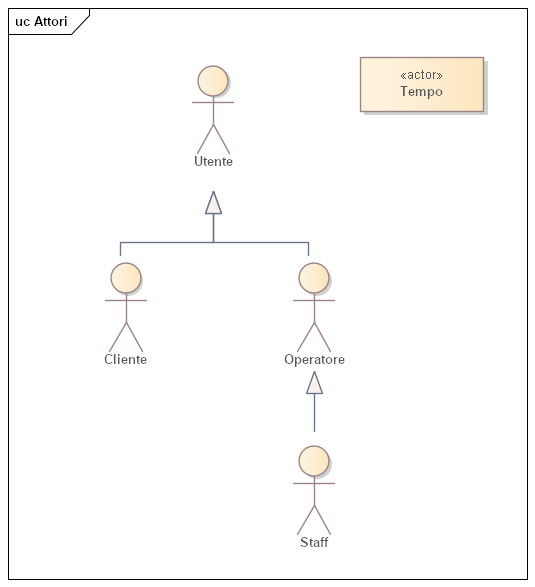
\includegraphics[width=1\textwidth]{Attori}
\end{figure*}

\newsection{Matrice di Mapping}

\newchapter{Analisi}

\newchapter{Progettazione}

\end{document}
